% RECUEIL DES FIGURES NATIVES — TikZ v1 (fusion des planches [bi], 100 % coraniques)
% Une planche par page (multi=tikzpicture). Sources absorbées : les 10 FIGURES_*_TIKZ_v1 natives
% du FP + FIGURES_GLOBE_ECUME_S1 (session feuille d'audit S1). Compiler : xelatex x2.
\documentclass[multi={tikzpicture},border=8pt]{standalone}
\usepackage{fontspec}\usepackage{amsmath}\usepackage{amssymb}\usepackage{tikz}
\usetikzlibrary{arrows.meta,calc,decorations.pathreplacing,decorations.text}
\newfontfamily\arab[Script=Arabic]{FreeSerif}
\newfontfamily\arAm[Script=Arabic,Scale=1.16]{Amiri Quran}
\protected\def\ar#1{\ifmmode\mbox{\normalfont\arAm #1}\else{\normalfont\arAm #1}\fi}
\newcommand{\Sx}[1]{\ensuremath{\mathrm{S}_{#1}}}
\definecolor{paper}{rgb}{0.995,0.992,0.982}
\definecolor{goldlite}{rgb}{0.93,0.90,0.78}
\definecolor{credit}{rgb}{0.11,0.40,0.22}
\definecolor{debit}{rgb}{0.55,0.12,0.12}
\definecolor{ink}{rgb}{0.17,0.14,0.10}
\definecolor{gold}{rgb}{0.61,0.48,0.13}
\definecolor{wAllah}{rgb}{0.69,0.48,0.18}
\definecolor{wBism}{rgb}{0.18,0.43,0.56}
\definecolor{wRahim}{rgb}{0.54,0.29,0.42}
\definecolor{wRahman}{rgb}{0.35,0.49,0.24}
\definecolor{vortg}{rgb}{0.35,0.49,0.24}
\begin{document}
% ================= PLANCHE 0 - L'INDEX =================
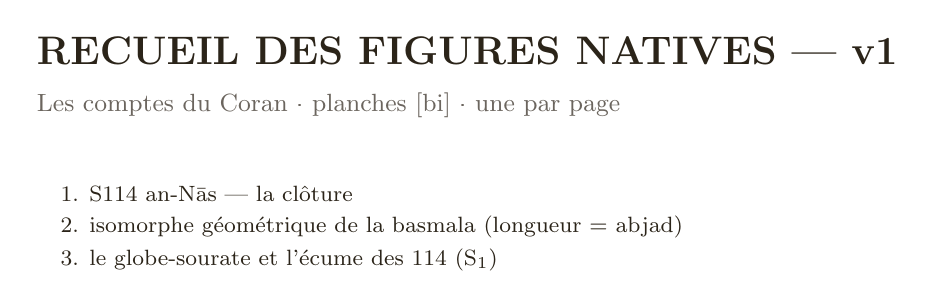
\begin{tikzpicture}
\node[anchor=west,font=\Large\bfseries,text=ink] at (0,0) {RECUEIL DES FIGURES NATIVES — v1};
\node[anchor=west,font=\small,text=ink!70] at (0,-0.7) {Les comptes du Coran · planches [bi] · une par page};
\node[anchor=west,font=\footnotesize,text=ink] at (0.3,-1.82) {1. S114 an-Nās — la clôture};
\node[anchor=west,font=\footnotesize,text=ink] at (0.3,-2.24) {2. isomorphe géométrique de la basmala (longueur $=$ abjad)};
\node[anchor=west,font=\footnotesize,text=ink] at (0.3,-2.66) {3. le globe-sourate et l'écume des 114 (\Sx{1})};
\end{tikzpicture}

% ================= PLANCHE : S114 an-Nās — la clôture — source : FIGURES_S114_ANNAS_TIKZ_v1.tex =================
% =====================================================================
% FIGURES_S114_ANNAS_TIKZ_v1.tex
% S.114 = an-Nās (la clôture, le bord du Livre). TikZ pur.
%
%   LA CLÔTURE : la 114e et dernière sourate ; profondeur 7 au cycle (le bord) ;
%     le dernier mot du Mushaf est الناس (an-nās). Le Voyage se referme ici.
%   LE BIVALENT : al-Fātiḥa (S.1, le seuil, prof 0, le centre/attracteur) <-> an-Nās
%     (S.114, la clôture, prof 7, le bord) — les deux extrémités du Mushaf (cœur->bord).
%   DONNÉES : source/feuille (deg_in=0) ; apex_verset=2 ; pointe -> S.2 ; nV=6 ;
%     ΣJ=5687 ; m=-1. Voyage : 114->2->70->3->33->20->88->1 (7 pas, le bord rejoint l'œil).
%   JUMELLE DE S.96 (al-'Alaq) : toutes deux prof 7, apex 2, pointe -> S.2 — la première
%     révélation et la dernière sourate se rejoignent en al-Baqara.
%   LE TRISKEL DES NOMS (v.1-3) : رب الناس (rabb=202) / ملك الناس (malik=90) /
%     اله الناس (ilāh=36) — et اله = 36 = T8 (« Dieu des hommes » pèse le nombre des connexions).
%   114 = 6·19 = 113+1 (le compte du manifeste, achevé).
%   LE REFUGE : min al-jinnati wa-n-nās (contre le waswās al-khannās).
%
% AUDIT [bi] — RECOMPTÉ : 01_DATA_toniques_114_apex_P2 (f(114)=2, apex=2, prof 7,
%   deg_in=0) ; 01_DATA_jummal_114_par_verset (nV=6, J(S.114)=5687, m=-1) ;
%   abjad mashriqī : الناس=142, رب=202, ملك=90, اله=36, وسواس=133, خناس=711.
%
% STATUTS : deg_in/apex/profondeur/J/nV/Voyage et abjad [bi] ;
%   bivalent seuil/bord, triskel des Noms et اله=36=T8 = lecture [R3].
%
% /!\ MOTEUR : XeLaTeX (ou LuaLaTeX) — arabe via fontspec.
%
% ---- PRÉAMBULE (XeLaTeX), une fois ----
% \usepackage{fontspec}\newfontfamily\arab[Script=Arabic]{FreeSerif}
% \usepackage{amsmath,amssymb,tikz}\usetikzlibrary{arrows.meta,calc}
% \definecolor{ink}{rgb}{0.17,0.14,0.10}\definecolor{gold}{rgb}{0.61,0.48,0.13}
\tikzset{
 pole/.style={circle,draw=gold,line width=1.3pt,fill=gold!20,inner sep=1pt,minimum size=0.9cm,text=ink,font=\bfseries},
 nm/.style={draw=gold,line width=0.9pt,rounded corners=4pt,fill=gold!13,inner sep=4pt,align=center,text=ink,font=\small,minimum width=1.7cm},
 rd/.style={ink,font=\footnotesize,anchor=west,text width=6.8cm},
 seal/.style={draw=gold,line width=1.1pt,rounded corners=4pt,fill=gold!14,inner sep=6pt,align=center,text=ink,font=\scriptsize,text width=13.4cm}}
% --------------------------------------
% \caption{S.114 (an-Nās), la clôture : la dernière sourate, le bord du Mushaf
%   (prof.\ 7), source ($\deg_{\rm in}=0$, apex 2, $\to$ S.2), jumelle de S.96 ;
%   le bivalent al-Fātiḥa$\leftrightarrow$an-Nās (cœur$\to$bord) ; le triskel des Noms
%   (rabb 202 / malik 90 / ilāh $=36=T_8$) ; $114=6\cdot19=113+1$.}

\begin{tikzpicture}[font=\sffamily]
\node[ink,font=\itshape\Large] at (7.2,9.1) {S.114 --- an-Nās ({\normalfont\arab الناس}) : la clôture, le bord du Livre};
\node[ink,font=\small\itshape] at (7.2,8.6) {la dernière sourate --- profondeur 7 (le bord) ; le dernier mot du Mushaf est {\normalfont\arab الناس}};
% ===== le bivalent al-Fatiha <-> an-Nas =====
\node[pole] (s1) at (1.7,7.35) {S.1};
\node[ink,font=\scriptsize,align=center] at (1.7,6.62) {al-Fātiḥa\\ le seuil --- prof 0};
\node[pole] (s114) at (5.7,7.35) {S.114};
\node[ink,font=\scriptsize,align=center] at (5.7,6.62) {an-Nās\\ la clôture --- prof 7};
\draw[gold,{Stealth[length=2mm]}-{Stealth[length=2mm]},line width=0.9pt,dash pattern=on 2.5pt off 2pt] (s1) -- (s114);
\node[ink,font=\scriptsize] at (3.7,7.62) {le Mushaf : du cœur au bord};
% ===== le triskel des Noms (v.1-3) =====
\node[ink,font=\footnotesize\bfseries] at (3.5,5.75) {Le triskel des Noms (v.1--3)};
\node[nm] (rabb) at (3.5,5.0) {{\arab رب الناس}\\ $202$};
\node[nm] (malik) at (2.15,3.85) {{\arab ملك الناس}\\ $90$};
\node[nm] (ilah) at (4.85,3.85) {{\arab اله الناس}\\ $\mathbf{36}$};
\draw[gold!75,-{Stealth[length=1.6mm]},line width=0.7pt] (rabb) to[bend right=16] (malik);
\draw[gold!75,-{Stealth[length=1.6mm]},line width=0.7pt] (malik) to[bend right=16] (ilah);
\draw[gold!75,-{Stealth[length=1.6mm]},line width=0.7pt] (ilah) to[bend right=16] (rabb);
\node[gold!85!black,font=\scriptsize,align=center] at (3.5,2.95) {{\arab اله} $=36=T_8$ (les connexions)};
% ===== 114 =====
\node[ink,font=\footnotesize,align=center] at (3.5,2.05) {$114 = 6\cdot19 = 113+1$\\ {\scriptsize le compte du manifeste, achevé}};
% ===== lecture (droite) =====
\node[rd] at (7.55,7.5) {\textbf{La dernière sourate} (la 114\textsuperscript{e}) : $nV=6$ ; $\Sigma J=5687$ ; $m=-1$};
\node[rd] at (7.55,6.75) {\textbf{Source} (feuille) : deg$_{\mathrm{in}}=0$ ; apex $=$ v.2 ; pointe $\to$ S.2};
\node[rd] at (7.55,5.85) {\textbf{Jumelle de S.96} (al-'Alaq) : toutes deux prof 7, apex 2, $\to$ S.2 --- la première révélation et la dernière sourate se rejoignent en al-Baqara};
\node[rd] at (7.55,4.7) {\textbf{Voyage} : $114\to2\to70\to3\to33\to20\to88\to1$ (7 pas --- le bord rejoint l'œil)};
\node[rd] at (7.55,3.75) {\textbf{Le refuge} : \emph{min al-jinnati wa-n-nās} (contre le waswās al-khannās) --- {\arab الناس} clôt aussi le Mushaf (son dernier mot)};
% ===== sceau =====
\node[seal] at (7.2,1.0) {la clôture du Mushaf --- le dernier mot {\arab الناس} ; \ al-Fātiḥa (le seuil, prof 0) $\leftrightarrow$ an-Nās (le bord, prof 7) ; \ le Voyage se referme \quad·\quad \texttt{[bi]}};
\end{tikzpicture}

% ================= PLANCHE : isomorphe géométrique de la basmala (longueur $=$ abjad) — source : FIGURES_BASMALA_ISOMORPHE_TIKZ_v1.tex =================
% =====================================================================
% FIGURES_BASMALA_ISOMORPHE_TIKZ_v1.tex
% Isomorphe géométrique de la basmala : longueur de segment = valeur abjad.
% Échelle EXACTE, réversible : mesurer un segment = lire sa valeur ;
% un bord de mot = le total courant (cumul). Superposable sur l'arithmétique
% PAR CONSTRUCTION — ce que le tracé thuluth n'est pas (projection à sens unique).
%
%   بسم=102 · الله=66 · الرحمن=329 · الرحيم=289  ->  ΣJ = 786 = 2·3·131 (4 mots, 19 lettres).
%   cumuls (droite->gauche) : 0,2,62,102,103,133,163,168,169,199,399,407,447,
%     497,498,528,728,736,746,786.
%   charges des mots : بسم 0 · الله 0 · الرحمن −1 · الرحيم +1  (somme 0).
%
% AUDIT [bi] — RECOMPTÉ (abjad mashriqī sur le rasm de 1:1, harakāt=0) :
%   19 lettres porteuses ; Σ largeurs = 786 ; lettre<->valeur bijectif sur le
%   sous-alphabet employé (ا ب ه ح ي ل م ن س ر, valeurs distinctes) ; cumul<->valeurs
%   par différences premières. La table abjad N'EST PAS globalement injective
%   (1←{ا,ء,أ,إ,آ}, 5←{ه,ة}, 6←{و,ؤ}, 10←{ي,ئ,ى}) : la réversibilité tient à CE rasm.
%
% /!\ MOTEUR : XeLaTeX (ou LuaLaTeX) — arabe via fontspec.
%
% ---- PRÉAMBULE (XeLaTeX), une fois ----
% \usepackage{fontspec}\newfontfamily\arab[Script=Arabic]{FreeSerif}
% \usepackage{amsmath,amssymb,tikz}\usetikzlibrary{calc,decorations.pathreplacing}
% \definecolor{ink}{rgb}{0.17,0.14,0.10}
% \definecolor{wBism}{rgb}{0.18,0.43,0.56}
% \definecolor{wAllah}{rgb}{0.69,0.48,0.18}
% \definecolor{wRahman}{rgb}{0.35,0.49,0.24}
% \definecolor{wRahim}{rgb}{0.54,0.29,0.42}
% --------------------------------------
% \caption{Isomorphe géométrique de la basmala : chaque segment a pour longueur
%   la valeur abjad de sa lettre (échelle exacte). La suite des lettres, celle des
%   valeurs et la trajectoire cumulée $2\!\to\!62\!\to\!\dots\!\to\!786$ sont en
%   bijection (réversibles, superposables) ; $786=2\cdot3\cdot131$. Le tracé
%   calligraphique, lui, n'est lié à son nombre que par une projection.}

\providecolor{wBism}{rgb}{0.18,0.43,0.56}
\providecolor{wAllah}{rgb}{0.69,0.48,0.18}
\providecolor{wRahman}{rgb}{0.35,0.49,0.24}
\providecolor{wRahim}{rgb}{0.54,0.29,0.42}
\providecolor{ink}{rgb}{0.17,0.14,0.10}
\begin{tikzpicture}[x=1cm,y=1cm]
\node[ink,font=\large] at (7.000,2.45){Isomorphe géométrique de la basmala — échelle exacte : longueur = valeur abjad};
\node[ink,font=\small\itshape] at (7.000,2.12){réversible et superposable sur l'arithmétique (mesurer un segment $=$ lire sa valeur ; bord de mot $=$ total courant)};
\draw[->,gray] (13.40,1.62)--(11.90,1.62);
\node[gray,font=\scriptsize,anchor=south] at (12.65,1.66){lecture (droite$\to$gauche)};
\fill[wBism!30,draw=white,line width=0.4pt] (13.964,0) rectangle (14.000,0.9);
\fill[wBism!50,draw=white,line width=0.4pt] (12.896,0) rectangle (13.964,0.9);
\fill[wBism!30,draw=white,line width=0.4pt] (12.183,0) rectangle (12.896,0.9);
\fill[wAllah!50,draw=white,line width=0.4pt] (12.165,0) rectangle (12.183,0.9);
\fill[wAllah!30,draw=white,line width=0.4pt] (11.631,0) rectangle (12.165,0.9);
\fill[wAllah!50,draw=white,line width=0.4pt] (11.097,0) rectangle (11.631,0.9);
\fill[wAllah!30,draw=white,line width=0.4pt] (11.008,0) rectangle (11.097,0.9);
\fill[wRahman!50,draw=white,line width=0.4pt] (10.990,0) rectangle (11.008,0.9);
\fill[wRahman!30,draw=white,line width=0.4pt] (10.455,0) rectangle (10.990,0.9);
\fill[wRahman!50,draw=white,line width=0.4pt] (6.893,0) rectangle (10.455,0.9);
\fill[wRahman!30,draw=white,line width=0.4pt] (6.751,0) rectangle (6.893,0.9);
\fill[wRahman!50,draw=white,line width=0.4pt] (6.038,0) rectangle (6.751,0.9);
\fill[wRahman!30,draw=white,line width=0.4pt] (5.148,0) rectangle (6.038,0.9);
\fill[wRahim!50,draw=white,line width=0.4pt] (5.130,0) rectangle (5.148,0.9);
\fill[wRahim!30,draw=white,line width=0.4pt] (4.595,0) rectangle (5.130,0.9);
\fill[wRahim!50,draw=white,line width=0.4pt] (1.033,0) rectangle (4.595,0.9);
\fill[wRahim!30,draw=white,line width=0.4pt] (0.891,0) rectangle (1.033,0.9);
\fill[wRahim!50,draw=white,line width=0.4pt] (0.712,0) rectangle (0.891,0.9);
\fill[wRahim!30,draw=white,line width=0.4pt] (0.000,0) rectangle (0.712,0.9);
\draw[gray!60,line width=0.3pt] (13.982,0.9)--(13.982,1.38);
\node[font=\small,text=wBism] at (13.982,1.42){\arab ب};
\node[font=\tiny,text=ink] at (13.982,1.62){$2$};
\node[font=\large,text=wBism] at (13.430,1.18){\arab س};
\node[font=\small,text=white] at (13.430,0.45){$60$};
\node[font=\large,text=wBism] at (12.539,1.18){\arab م};
\node[font=\small,text=white] at (12.539,0.45){$40$};
\draw[gray!60,line width=0.3pt] (12.174,0.9)--(12.174,1.38);
\node[font=\small,text=wAllah] at (12.174,1.42){\arab ا};
\node[font=\tiny,text=ink] at (12.174,1.62){$1$};
\node[font=\normalsize,text=wAllah] at (11.898,1.18){\arab ل};
\node[font=\scriptsize,text=ink] at (11.898,1.00){$30$};
\node[font=\normalsize,text=wAllah] at (11.364,1.18){\arab ل};
\node[font=\scriptsize,text=ink] at (11.364,1.00){$30$};
\draw[gray!60,line width=0.3pt] (11.052,0.9)--(11.052,1.38);
\node[font=\small,text=wAllah] at (11.052,1.42){\arab ه};
\node[font=\tiny,text=ink] at (11.052,1.62){$5$};
\draw[gray!60,line width=0.3pt] (10.999,0.9)--(10.999,1.74);
\node[font=\small,text=wRahman] at (10.999,1.78){\arab ا};
\node[font=\tiny,text=ink] at (10.999,1.98){$1$};
\node[font=\normalsize,text=wRahman] at (10.723,1.18){\arab ل};
\node[font=\scriptsize,text=ink] at (10.723,1.00){$30$};
\node[font=\large,text=wRahman] at (8.674,1.18){\arab ر};
\node[font=\small,text=white] at (8.674,0.45){$200$};
\draw[gray!60,line width=0.3pt] (6.822,0.9)--(6.822,1.38);
\node[font=\small,text=wRahman] at (6.822,1.42){\arab ح};
\node[font=\tiny,text=ink] at (6.822,1.62){$8$};
\node[font=\large,text=wRahman] at (6.394,1.18){\arab م};
\node[font=\small,text=white] at (6.394,0.45){$40$};
\node[font=\large,text=wRahman] at (5.593,1.18){\arab ن};
\node[font=\small,text=white] at (5.593,0.45){$50$};
\draw[gray!60,line width=0.3pt] (5.139,0.9)--(5.139,1.38);
\node[font=\small,text=wRahim] at (5.139,1.42){\arab ا};
\node[font=\tiny,text=ink] at (5.139,1.62){$1$};
\node[font=\normalsize,text=wRahim] at (4.863,1.18){\arab ل};
\node[font=\scriptsize,text=ink] at (4.863,1.00){$30$};
\node[font=\large,text=wRahim] at (2.814,1.18){\arab ر};
\node[font=\small,text=white] at (2.814,0.45){$200$};
\draw[gray!60,line width=0.3pt] (0.962,0.9)--(0.962,1.38);
\node[font=\small,text=wRahim] at (0.962,1.42){\arab ح};
\node[font=\tiny,text=ink] at (0.962,1.62){$8$};
\draw[gray!60,line width=0.3pt] (0.802,0.9)--(0.802,1.74);
\node[font=\small,text=wRahim] at (0.802,1.78){\arab ي};
\node[font=\tiny,text=ink] at (0.802,1.98){$10$};
\node[font=\large,text=wRahim] at (0.356,1.18){\arab م};
\node[font=\small,text=white] at (0.356,0.45){$40$};
\draw[ink,line width=0.6pt] (0,0)--(14.000,0);
\draw[ink,line width=0.6pt] (14.000,0)--(14.000,-0.16);
\node[font=\scriptsize,text=ink] at (14.000,-0.32){$0$};
\draw[ink,line width=0.3pt] (13.964,0)--(13.964,-0.08);
\draw[ink,line width=0.3pt] (12.896,0)--(12.896,-0.08);
\draw[ink,line width=0.6pt] (12.183,0)--(12.183,-0.16);
\node[font=\scriptsize,text=ink] at (12.183,-0.32){$102$};
\draw[ink,line width=0.3pt] (12.165,0)--(12.165,-0.08);
\draw[ink,line width=0.3pt] (11.631,0)--(11.631,-0.08);
\draw[ink,line width=0.3pt] (11.097,0)--(11.097,-0.08);
\draw[ink,line width=0.6pt] (11.008,0)--(11.008,-0.16);
\node[font=\scriptsize,text=ink] at (11.008,-0.32){$168$};
\draw[ink,line width=0.3pt] (10.990,0)--(10.990,-0.08);
\draw[ink,line width=0.3pt] (10.455,0)--(10.455,-0.08);
\draw[ink,line width=0.3pt] (6.893,0)--(6.893,-0.08);
\draw[ink,line width=0.3pt] (6.751,0)--(6.751,-0.08);
\draw[ink,line width=0.3pt] (6.038,0)--(6.038,-0.08);
\draw[ink,line width=0.6pt] (5.148,0)--(5.148,-0.16);
\node[font=\scriptsize,text=ink] at (5.148,-0.32){$497$};
\draw[ink,line width=0.3pt] (5.130,0)--(5.130,-0.08);
\draw[ink,line width=0.3pt] (4.595,0)--(4.595,-0.08);
\draw[ink,line width=0.3pt] (1.033,0)--(1.033,-0.08);
\draw[ink,line width=0.3pt] (0.891,0)--(0.891,-0.08);
\draw[ink,line width=0.3pt] (0.712,0)--(0.712,-0.08);
\draw[ink,line width=0.6pt] (0.000,0)--(0.000,-0.16);
\node[font=\scriptsize,text=ink] at (0.000,-0.32){$786$};
\node[font=\large,text=wRahim,anchor=south] at (0.0,1.97){$786$};
\node[font=\scriptsize,text=wRahim,anchor=north] at (0.0,1.97){$=2\cdot3\cdot131$, charge $0$};
\draw[decorate,decoration={brace,amplitude=4pt,mirror},ink,line width=0.6pt] (14.000,-0.46)--(12.183,-0.46);
\node[font=\normalsize,text=wBism] at (13.092,-0.86){\arab بسم};
\node[font=\scriptsize,text=ink] at (13.092,-1.12){bi-smi};
\node[font=\scriptsize,text=ink!70] at (13.092,-1.34){$102$, charge $0$};
\draw[decorate,decoration={brace,amplitude=4pt,mirror},ink,line width=0.6pt] (12.183,-0.46)--(11.008,-0.46);
\node[font=\normalsize,text=wAllah] at (11.595,-0.86){\arab الله};
\node[font=\scriptsize,text=ink] at (11.595,-1.12){All\=ah};
\node[font=\scriptsize,text=ink!70] at (11.595,-1.34){$66$, charge $0$};
\draw[decorate,decoration={brace,amplitude=4pt,mirror},ink,line width=0.6pt] (11.008,-0.46)--(5.148,-0.46);
\node[font=\normalsize,text=wRahman] at (8.078,-0.86){\arab الرحمن};
\node[font=\scriptsize,text=ink] at (8.078,-1.12){ar-Ra\d{h}m\=an};
\node[font=\scriptsize,text=ink!70] at (8.078,-1.34){$329$, charge $-1$};
\draw[decorate,decoration={brace,amplitude=4pt,mirror},ink,line width=0.6pt] (5.148,-0.46)--(0.000,-0.46);
\node[font=\normalsize,text=wRahim] at (2.574,-0.86){\arab الرحيم};
\node[font=\scriptsize,text=ink] at (2.574,-1.12){ar-Ra\d{h}\=im};
\node[font=\scriptsize,text=ink!70] at (2.574,-1.34){$289$, charge $+1$};
\node[ink!70,font=\scriptsize,anchor=west,align=left] at (0,-1.80){Le tracé thuluth n'est pas superposable à son nombre (projection à sens unique) ; cette figure l'est, par construction.\\ Échelle : 1 unité abjad $=0.0178$\,cm. 19 segments ; somme des largeurs $=786$.};
\end{tikzpicture}

% ================= PLANCHE : le globe-sourate et l'écume des 114 =================
\begin{tikzpicture}[font=\scriptsize]
%%%%%%%%%%%%%%%%%%%%%%%%%%%%%%%%%%%%%%%%%%%%%%% PANNEAU A : le globe-sourate
\begin{scope}[xshift=0cm]
% ombre portee
\fill[black!10] (0.12,-2.72) ellipse (2.35 and 0.30);
% boule pleine (surface externe, dehors = zahir)
\shade[shading=radial,inner color=paper,outer color=goldlite!75!black!30] (0,0) circle (2.6);
\fill[white,opacity=0.45] (-0.85,1.15) ellipse (0.95 and 0.62); % lumiere
% secteur decoupe (bas-droite) : les couches concentriques (portes emboitees)
\begin{scope}
  \fill[goldlite!45] (0,0) -- (-18:2.6)  arc (-18:-108:2.6)  -- cycle; % V1+V7 = 6796
  \fill[black!8]     (0,0) -- (-18:1.95) arc (-18:-108:1.95) -- cycle; % V2+V6 = 1655
  \fill[debit!11]    (0,0) -- (-18:1.30) arc (-18:-108:1.30) -- cycle; % V3+V5 = 1454
  \fill[debit!22]    (0,0) -- (-18:0.65) arc (-18:-108:0.65) -- cycle; % V4 = 242
  \fill[black,opacity=0.05] (0,0) -- (-18:2.6) arc (-18:-108:2.6) -- cycle; % profondeur
  \draw[ink!55,line width=0.5pt] (0,0) -- (-18:2.6);
  \draw[ink!55,line width=0.5pt] (0,0) -- (-108:2.6);
  \foreach \r in {0.65,1.30,1.95} \draw[ink!30,line width=0.35pt] (-18:\r) arc (-18:-108:\r);
\end{scope}
% enclos dore
\draw[gold,line width=1.5pt] (0,0) circle (2.6);
% la porte (bab) sur le limbe, angle 32
\begin{scope}[rotate=32]
  \fill[goldlite!85] (2.28,-0.34) rectangle (2.6,0.34);
  \draw[gold,line width=1.2pt] (2.6,-0.34) -- (2.28,-0.34) -- (2.28,0.34) -- (2.6,0.34);
  \draw[gold,line width=1.5pt] (2.60,-0.34) -- ++(0.42,0.22); % battant entrouvert
\end{scope}
\foreach \a in {22,32,42} \draw[gold!75,line width=0.45pt] (\a:2.72) -- (\a:2.98); % halo
% etiquettes panneau A
\node[ink!75] at (0.95,1.45) {\ar{ظاهر} \,\emph{(dehors)}};
\node[ink!85] at (-95:1.72) {\ar{باطن} \,\emph{(dedans)}};
\node[gold!62!ink,font=\tiny,anchor=east,align=right] at (-2.95,0.55) {\ar{سورة} $=271=$ \ar{المر}\\ l'enclos};
\draw[gold!60,line width=0.45pt] (-2.9,0.48) -- (169:2.64);
% masses des couches
\node[ink!80,font=\tiny] at (-63:2.28) {6796};
\node[ink!80,font=\tiny] at (-63:1.63) {1655};
\node[ink!80,font=\tiny] at (-63:0.98) {1454};
\node[debit!80!ink,font=\tiny] at (-63:0.36) {242};
% porte + cle
\node[gold!80!ink,align=left,font=\tiny,anchor=west] at (3.05,1.75) {\ar{باب} $=5$ (57:13)\\ la porte};
\draw[-Stealth,gold!80!ink,line width=0.5pt] (3.0,1.72) -- (32:2.75);
\node[ink!75,align=left,font=\tiny,anchor=west] at (3.05,0.9) {la cl\'e : $\varphi_1=786$\\ tourn\'ee par \ar{باسم} $=103$};
\draw[-Stealth,ink!55,line width=0.5pt] (3.0,1.02) to[bend right=10] (30:2.68);
\node[ink,font=\footnotesize\bfseries] at (0.2,-3.35) {le globe-sourate \Sx{1} — la coupe};
\end{scope}
%%%%%%%%%%%%%%%%%%%%%%%%%%%%%%%%%%%%%%%%%%%%%%% PANNEAU B : l'ecume du volume
\begin{scope}[xshift=9.6cm]
\fill[black!10] (0.10,-2.62) ellipse (2.45 and 0.28);
\begin{scope}
\clip (0,0) circle (2.45);
\tikzset{cellule/.style={draw=ink!40,line width=0.55pt,rounded corners=2.5pt,fill=paper}}
\path[cellule,fill=goldlite!55] (-0.73,-0.01) -- (-0.15,-0.75) -- (0.54,-0.32) -- (0.47,0.40) -- (-0.15,0.64) -- cycle;
\path[cellule,fill=black!5] (1.48,-0.77) -- (1.82,-0.78) -- (1.29,0.80) -- (1.02,0.81) -- (0.47,0.40) -- (0.54,-0.32) -- cycle;
\path[cellule,fill=credit!7] (0.59,1.55) -- (1.02,0.81) -- (0.47,0.40) -- (-0.15,0.64) -- (-0.40,1.34) -- (-0.38,1.39) -- cycle;
\path[cellule,fill=debit!7] (-2.03,0.85) -- (-0.40,1.34) -- (-0.15,0.64) -- (-0.73,-0.01) -- (-1.29,0.02) -- cycle;
\path[cellule,fill=black!7] (-1.29,0.02) -- (-0.73,-0.01) -- (-0.15,-0.75) -- (-0.22,-1.07) -- (-0.85,-1.35) -- (-1.47,-0.70) -- cycle;
\path[cellule,fill=credit!6] (-0.22,-1.07) -- (0.30,-1.63) -- (1.48,-0.77) -- (0.54,-0.32) -- (-0.15,-0.75) -- cycle;
\path[cellule,fill=debit!6] (2.31,1.46) -- (2.30,1.46) -- (1.29,0.80) -- (1.82,-0.78) -- (2.83,-1.25) -- (2.85,-1.25) -- cycle;
\path[cellule,fill=black!5] (1.00,2.44) -- (2.30,1.46) -- (1.29,0.80) -- (1.02,0.81) -- (0.59,1.55) -- cycle;
\path[cellule,fill=credit!5] (0.99,2.46) -- (-0.61,2.63) -- (-0.38,1.39) -- (0.59,1.55) -- (1.00,2.44) -- cycle;
\path[cellule,fill=debit!5] (-2.58,1.08) -- (-2.42,1.46) -- (-0.63,2.64) -- (-0.61,2.63) -- (-0.38,1.39) -- (-0.40,1.34) -- (-2.03,0.85) -- cycle;
\path[cellule,fill=black!6] (-2.79,0.99) -- (-2.38,-1.14) -- (-2.37,-1.14) -- (-1.47,-0.70) -- (-1.29,0.02) -- (-2.03,0.85) -- (-2.58,1.08) -- cycle;
\path[cellule,fill=credit!6] (-2.37,-1.14) -- (-1.35,-2.36) -- (-1.31,-2.34) -- (-0.85,-1.35) -- (-1.47,-0.70) -- cycle;
\path[cellule,fill=debit!6] (-0.85,-1.35) -- (-0.22,-1.07) -- (0.30,-1.63) -- (0.49,-2.70) -- (-1.31,-2.34) -- cycle;
\path[cellule,fill=black!5] (0.30,-1.63) -- (0.49,-2.70) -- (2.83,-1.25) -- (1.82,-0.78) -- (1.48,-0.77) -- cycle;
% highlights 3D
\foreach \x/\y in {-0.06/-0.01,1.06/0.10,0.35/1.05,-0.81/0.65,-0.89/-0.66,0.55/-0.99,1.60/0.30,1.14/1.51,0.20/1.94,-1.12/1.69,-1.85/-0.30,-1.45/-1.25,-0.36/-1.75,0.95/-1.50}
  \fill[white,opacity=0.26] (\x-0.12,\y+0.14) ellipse (0.18 and 0.09);
\end{scope}
\draw[ink!45,line width=0.8pt] (0,0) circle (2.45);
% S1 doree = la cellule centrale
\node[gold!80!ink,font=\bfseries\scriptsize] at (-0.06,-0.01) {$\mathrm{S}_1$};
% etiquettes panneau B
\node[ink!75,font=\tiny,align=left,anchor=west] at (2.65,1.5) {parois \textbf{partag\'ees} —\\ jamais d\'etach\'ees (\ar{جفاء})};
\draw[-Stealth,ink!55,line width=0.5pt] (2.62,1.45) -- (1.45,0.55);
\node[ink!75,font=\tiny,align=left,anchor=west] at (2.62,0.45) {\ar{بنيان مرصوص}\\ $=539=7^2{\cdot}11$};
\node[ink,font=\footnotesize\bfseries,align=center] at (0.1,-3.35) {le volume — « une \'ecume de \textbf{114} cellules soud\'ees »\\[-1pt] {\normalfont\tiny (\texttt{LE\_VOLUME}) — nou\'ee de 36 connexions ; \Sx{1} en est une}};
\end{scope}
%%%%%%%%%%%%%%%%%%%%%%%%%%%%%%%%%%%%%%%%%%%%%%% separation des echelles
\draw[ink!30,dashed] (5.15,-2.6) -- (5.15,2.9);
\node[ink!60,font=\tiny] at (4.85,-3.90) {— deux \'echelles, qui ne se m\'elangent pas (loi, r\`egle 6) —};
\end{tikzpicture}
\end{document}
